\clearpage
\newpage
\section{Cost Analysis}\label{sec:cost_analysis}
\paragraph{More powerful models are cost-efficient for instruction proposal} Despite higher per-token costs, we find larger, human-aligned models (models trained to follow human instructions \citep{ouyang2022training}) dominate the accuracy-cost frontier of \algname (Figure \ref{fig:cost-frontier}). Compared to smaller models not fined-tuned with human instructions, they tend to generate more concise instructions  (Figure \ref{fig:model-instr-len}), significantly reducing the cost of \algname scoring. Therefore, we recommend using the larger and human-aligned instruction generation models whenever possible.
% Instructions are limited to 50 tokens with 4 tokens of meta prompt overhead across all experiments, though the more capable models require much less. We argue with the benefits to conciseness, cost-efficiency of \algname, and higher accuracy, the larger human-aligned instruction generation models should be used when possible.

\paragraph{APE instructions are context condensers}
Although zero-shot instructions require more extensive sampling and scoring offline than in-context learning, they are token-efficient when amortized over a large number of inferences. In this light, we view the cost of \algname as a one-time overhead to distill a concise prompt from demonstrations. As shown in Figure \ref{fig:instr-ic-len}, \algname instructions reduce the number of prompt tokens by up to an order of magnitude compared to in-context learning. Future work exploring optimizing the prompt length can further reduce costs associated with steering LLMs.
\begin{figure}[th]
  \centering
  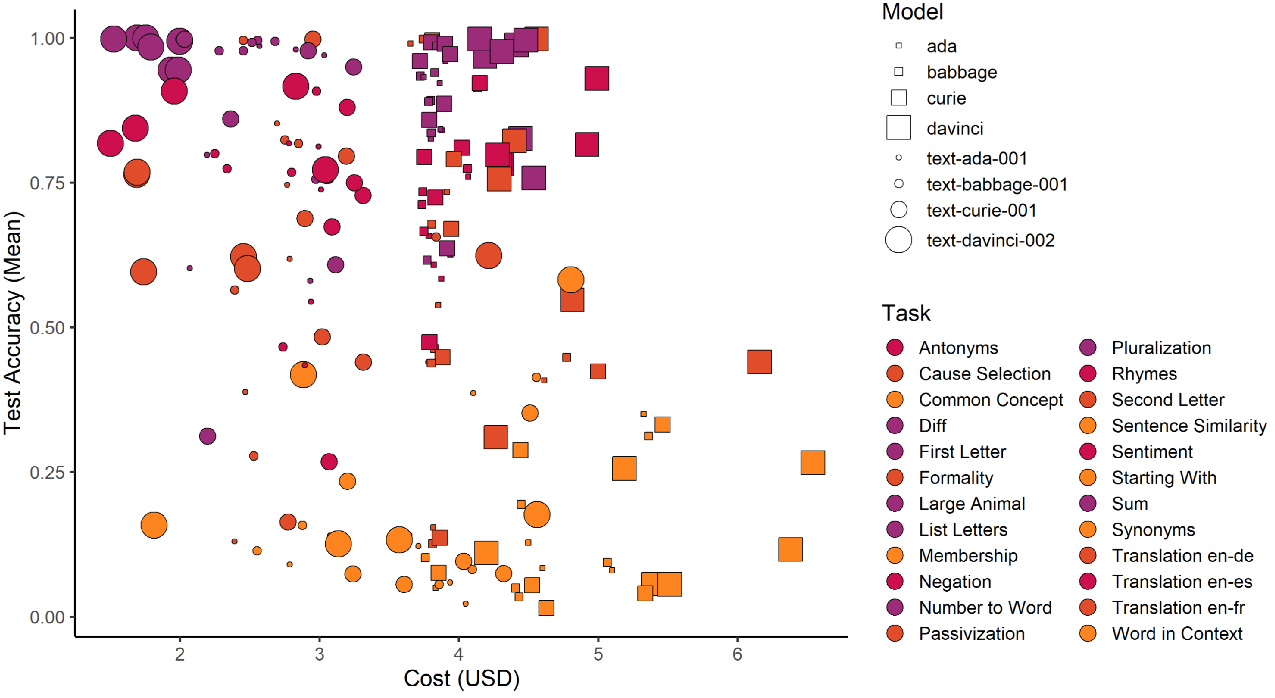
\includegraphics[width=0.95\linewidth]{figures/appendix/cost_frontier.pdf}
  \caption{The accuracy-cost frontier of \algname across eight OpenAI models. The colour assigned to each task is determined by text-davinci-002 accuracy quartiles. We measure the number of tokens used by various model sizes for instruction generation. We also measure the number of tokens used to score 250 generated instructions on ten validation input-output pairs on InstructGPT (i.e., text-davinci-002). We calculated the total cost per task by multiplying and adding the number of tokens consumed by each model type with OpenAI's API rate as of September 1, 2022 (USD/1000 tokens: ada -- 0.0004, babbage -- 0.0005, curie -- 0.0020, davinci -- 0.0200). Counter-intuitively, smaller models are more expensive. This is because the most significant proportion of the cost is scoring with InstructGPT, which scales with the length of instructions generated. Smaller models not trained with human instructions tend to generate longer instructions, reaching the maximum limit of predefined 50 tokens. Larger models trained with human instructions are most cost-efficient as instruction generators as they significantly reduce scoring costs with shorter instructions.}
  \label{fig:cost-frontier}
\end{figure}

\begin{figure}[th]
  \centering
  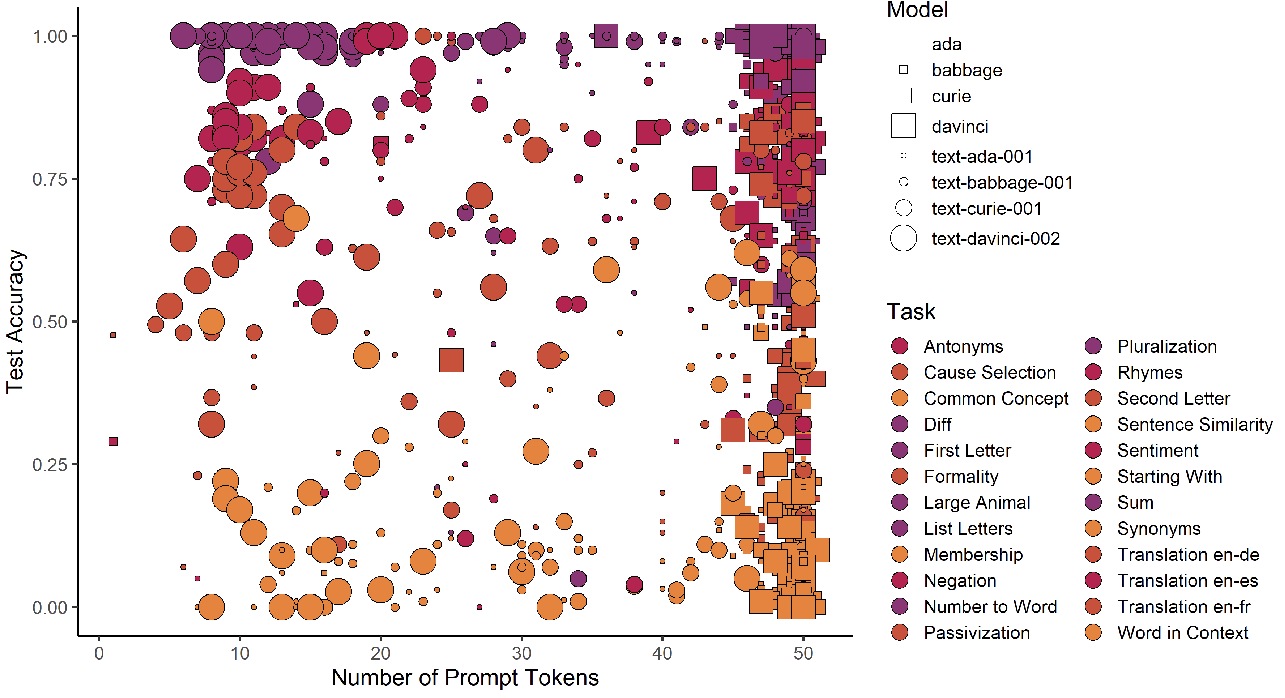
\includegraphics[width=0.95\linewidth]{figures/appendix/model_instr_len.pdf}
  \caption{The accuracy-length frontier of prompts generated across eight OpenAI models and 24 NLP tasks. Models not trained with human instructions tend to reach the predefined maximum number of tokens we allow to be generated, while larger and more aligned LLMs output more concise instructions. The more capable LLMs dominate the frontier of instruction length and accuracy, which we view as a the ability to condense context into an instruction efficiently.}
  \label{fig:model-instr-len}
\end{figure}

% ziwens fig 2
\begin{figure}[th]
  \centering
  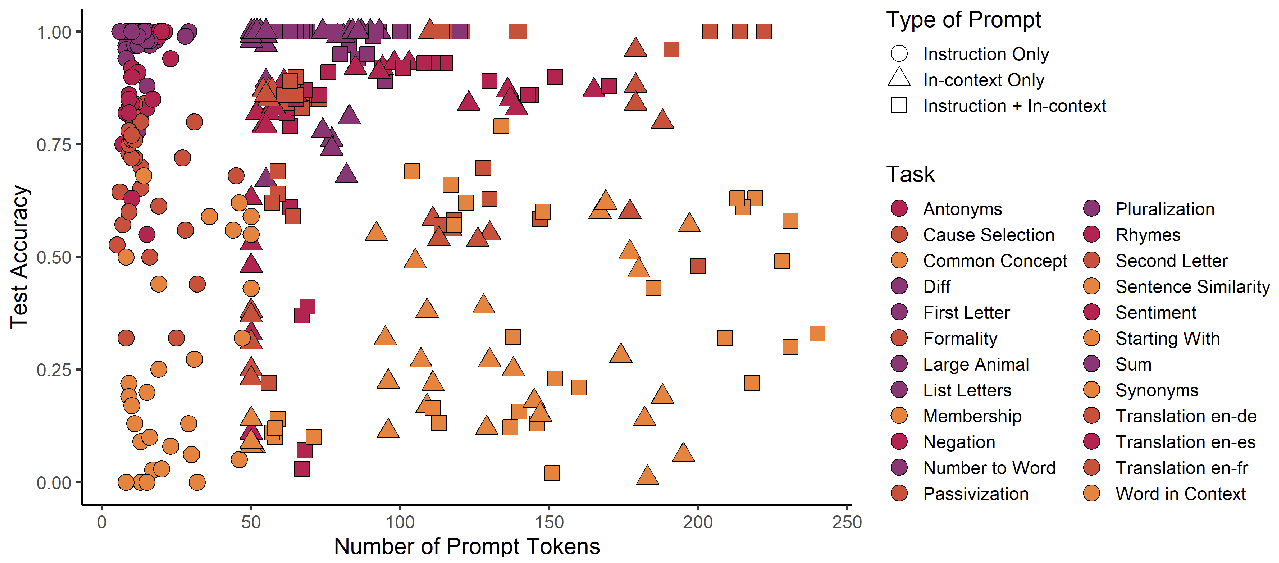
\includegraphics[width=0.95\linewidth]{figures/appendix/context_instr_len.pdf}
  \caption{Instructions found by \algname from InstructGPT are token efficient compared to using five in-context examples. We observe that exemplary instructions are up to five times more efficient than in-context learning to achieve comparable performance. Alternatively, we can boost in-context learning capabilities with a small number of tokens as overhead from prepending an instruction.}
  \label{fig:instr-ic-len}
\end{figure}
